\documentclass[titlepage, a4paper, 11pt, dvipdfmx]{jsarticle}
\usepackage{customstyle}

\title{\Huge【レポート\#4 CG法}
\date{\today}%日付
\author{\Large BV20036 \quad 大野 弘貴}%名前

\begin{document}
\maketitle
\pagenumbering{roman}
% \tableofcontents%目次が消したい場合はコメントアウト
\newpage
\pagenumbering{arabic}

%%%%%%%%%%%%%%%%%%%%%%%%%%%%%%%%%%%%%%%%%%%%%%%%%%%%%%%%%%%%%%%%%%%%%%%%%%%%%
%%%%%%%%%%%%%%%%%%%%%%%%%%%%%%%%%%%%%%%%%%%%%%%%%%%%%%%%%%%%%%%%%%%%%%%%%%%%%
%%%%%%%%%%%%%%%%%%%%%%%%%%%%%%%%%%%%%%%%%%%%%%%%%%%%%%%%%%%%%%%%%%%%%%%%%%%%%
%以下サンプル%ここから書き始めてください

%セクション(目次に表示されるのは初期設定では)
\section{レポート内容}
\begin{itembox}[l]{CG法}
下の行列$A_1, A_2$を係数行列とする連立一時方程式に対し、以下の条件のもとでCG法を適用し収束するまでの反復回数及び得られた近似解x\textasciitilde に対する相対残差2ノルム$ \| b - Ax$\textasciitilde $ \|_2/ \| b \|_2 $および真の解 x\textasciitilde との相対残差2ノルム$ \| x^* - x$\textasciitilde $ \|_2 $をもとめよ。さらに、横軸を反復回数縦軸(対数)を相対残差2ノルムとする収束履歴のグラフを作成し、得られた結果について考察せよ。
    \begin{itemize}
        \item 初期近似解:$x_0 = 0 $
        \item 行列サイズ:$ n = 100, 500$
        \item 最大反復回数:行列サイズ$n$に対し$2n$とする。
        \item 許容誤差:$\varepsilon = 10^{-12}$
        \item 収束反転条件:相対残差2ノルム
    \end{itemize}
    ($\| r_{k+1} \|_2$)
    \begin{itemize}
        \item 真の解:$ x^* = ( 1,1,\cdots,1 )^T $
        \item 右辺項: b = A * x \textasciitilde として作成せよ
    \end{itemize}
\end{itembox}
    \section{CG(Conjugate Gradient)法とは}

    \begin{itemize}
        \item  大規模で疎な正定値対称行列を係数行列とする連立一次方程式を解く反復法
        \item  非零成分の割合が非常に少ない行列 (⇔ 密行列)
        \item 大規模疎行列は偏微分方程式の数値計算 (離散化) でよくあらわれる
        \item 通常は, あらかじめ条件数を小さくするような「前処理」を行った CG 法がよく用いられる
        \begin{itemize}
            \item 不完全コレスキー分解前処理付き共役交配法 (ICCG 法)
        \end{itemize}
        \item 大規模疎行列の場合, 二次元配列に行列のすべての成分を格納するのではなく, 行列の非零成分のみを保持する疎行列格納形式が用いられる.
        \begin{itemize}
            \item CRS 形式, CCS 形式. COO 形式, $\cdots$
        \end{itemize}
    \end{itemize}

\section{実行結果}

\begin{table}[H]
\begin{tabular}{|l|ll|ll|llllllllllllllll}
\cline{1-5}
\multicolumn{1}{|r|}{} & \multicolumn{2}{l|}{$A_1$}                                       & \multicolumn{2}{l|}{$A_2$}                                       &  &  &  &  &  &  &  &  &  &  &  &  &  &  &  &  \\ \cline{1-5}
行列のサイズ                 & \multicolumn{1}{l|}{100}                              & 500      & \multicolumn{1}{l|}{100}                              & 500      &  &  &  &  &  &  &  &  &  &  &  &  &  &  &  &  \\ \cline{1-5}
反復回数                   & 40       & 39       & 39       & 266      &  &  &  &  &  &  &  &  &  &  &  &  &  &  &  &  \\ \cline{1-5}
相対残差2ノルム               & 7.19e-13 & 7.59e-13 & 8.27e-13 & 8.27e-13 &  &  &  &  &  &  &  &  &  &  &  &  &  &  &  &  \\ \cline{1-5}
相対誤差2ノルム               & 3.27e-12                        & 7.42e-12 & 2.17e-08             & 9.30e-07 &  &  &  &  &  &  &  &  &  &  &  &  &  &  &  &  \\ \cline{1-5}
\end{tabular}
\end{table}

\begin{figure}[H]
    \begin{center}%中央寄せ用
      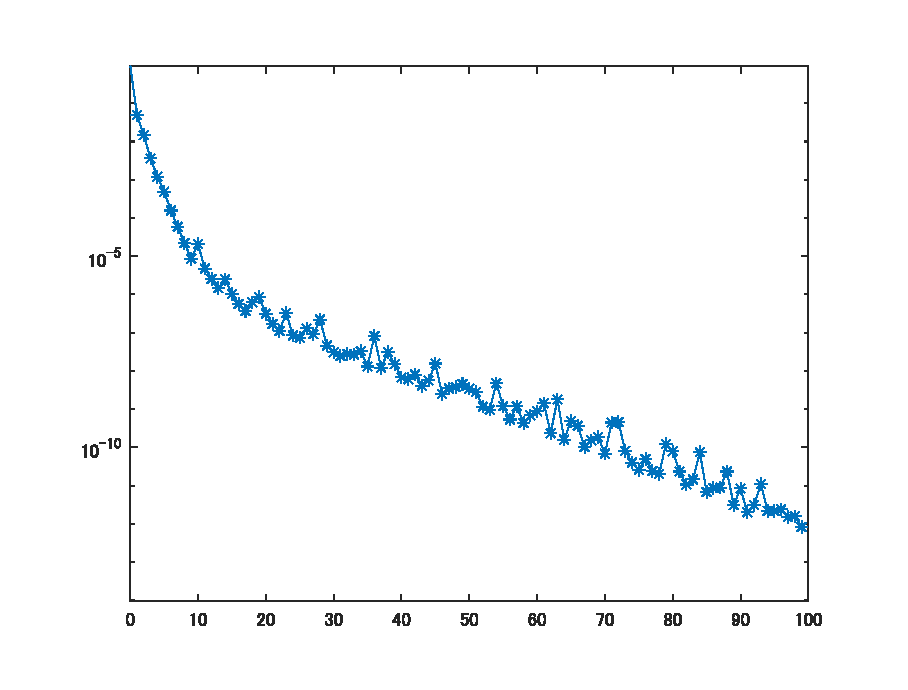
\includegraphics[width=13.5cm]{./graphics/CG/100.eps}
    \caption{$A_2$ n=100}
    \label{Label}%ラベル
    \end{center}
  \end{figure}

  \begin{figure}[H]
    \begin{center}%中央寄せ用
      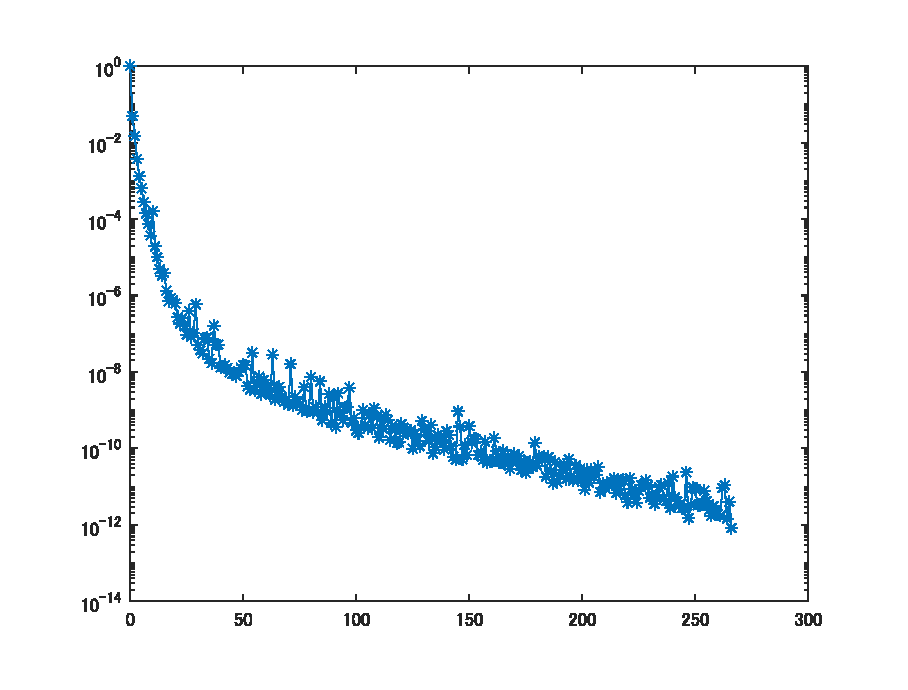
\includegraphics[width=13.5cm]{./graphics/CG/500.eps}
    \caption{$A_2$ n=500}
    \label{Label}%ラベル
    \end{center}
  \end{figure}

  \begin{figure}[H]
    \begin{center}%中央寄せ用
      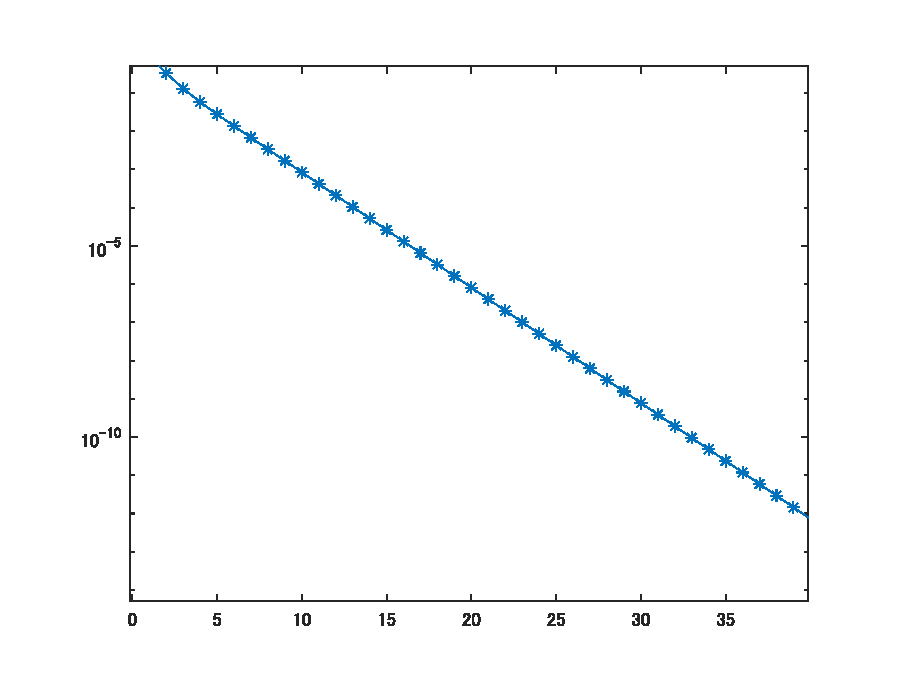
\includegraphics[width=13.5cm]{./graphics/CG/100rema.eps}
    \caption{$A_1$ n=100}
    \label{Label}%ラベル
    \end{center}
  \end{figure}


  \begin{figure}[H]
    \begin{center}%中央寄せ用
      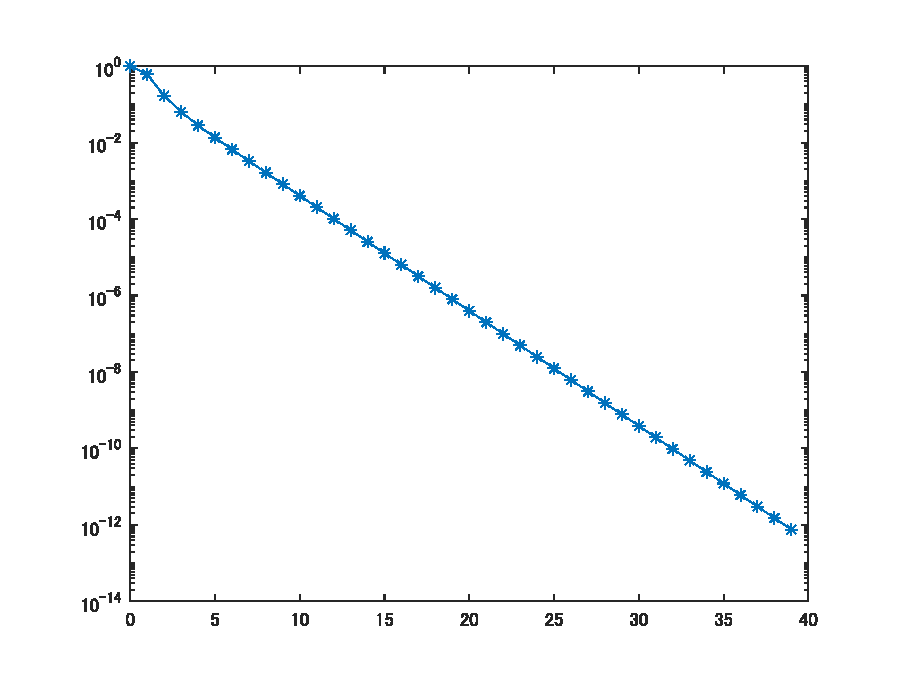
\includegraphics[width=13.5cm]{./graphics/CG/500rema.eps}
    \caption{$A_1$ n=500}
    \label{Label}%ラベル
    \end{center}
  \end{figure}

\section{考察}
$A_1$の行列はわかりやすく、nが多くなく成るほど線形に精度がよくなっていくことがわかった。対して$A_2$はnを増やすと徐々に精度がよくなっていくことは変わらないが、$A_2$とは違い線形ではなく、波が生じながら精度が良くなっている。
 また、相対誤差に関しては、行列が大きくなると要素数が増え計算が多くなることが原因なのか、行列を大きくしたほうが相対誤差も増えた。
\end{document}
